\subsection{Animation}
Um eine möglichst optimale Benutzerfreundlichkeit zu gewährleisten, soll der berechnete Stoss über eine Animation
auf dem Tisch dargestellt werden. Dies wird durch eine Übersetzung des physikalischen Simulationsmodells, wie in Kapitel
\ref{kap:physikalisches_system} beschrieben, erzielt.

Die Animation besteht aus Keyframes, zwischen welchen interpoliert werden kann. Das grundlegende Prinzip wird in Abbildung
\ref{fig:keyframe_animation} visualisiert. Auf der linken Seite wird der Zeitstrahl angegeben. Die Zeit schreitet in vertikaler
Richtung nach unten voran. Der rote Pfeil markiert den aktuellen Zeitpunkt, dieser liegt zwischen Keyframe 1 und Keyframe 2.
Der Status zu diesem Zeitpunkt kann durch Interpolation zwischen den genannten Keyframes berechnet werden.

\begin{figure}[h!]
    \begin{center}
        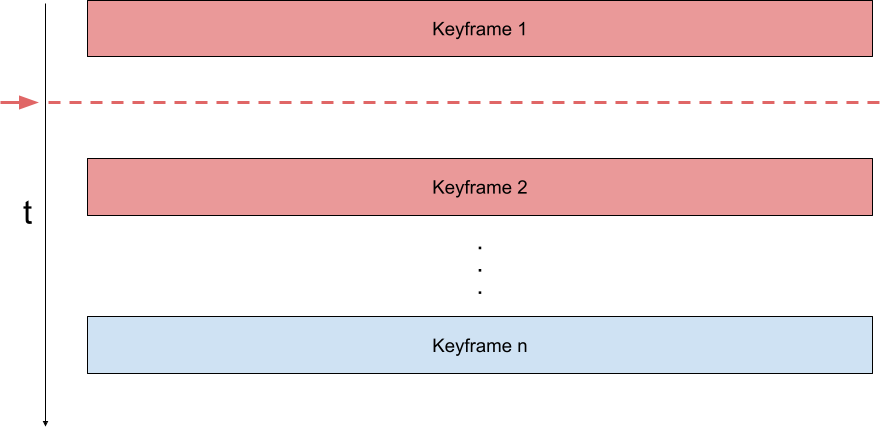
\includegraphics[width=0.6\linewidth]{../common/03_billiard_ai/resources/31_keyframe_animation.png}
    \end{center}
    \caption{Keyframe Animation}
    \label{fig:keyframe_animation}
\end{figure}

Das Animationsmodell wird anhand des Simulationsmodells abgeleitet. Dazu kann Abbildung
\ref{fig:simulationsmodell_keyframes} betrachtet werden. Wie in Kapitel \ref{kap:physikalisches_system} erklärt, besteht
das physikalische Simulationsmodell aus in Layern gruppierte Knoten. Diese Knoten haben jeweils eine Eingabe- wie auch
eine Ausgabeschicht. Eine Gruppierung dieser Knoten in einem Layer weist dadurch dieselbe Eigenschaft auf.

\begin{figure}[h!]
    \begin{center}
        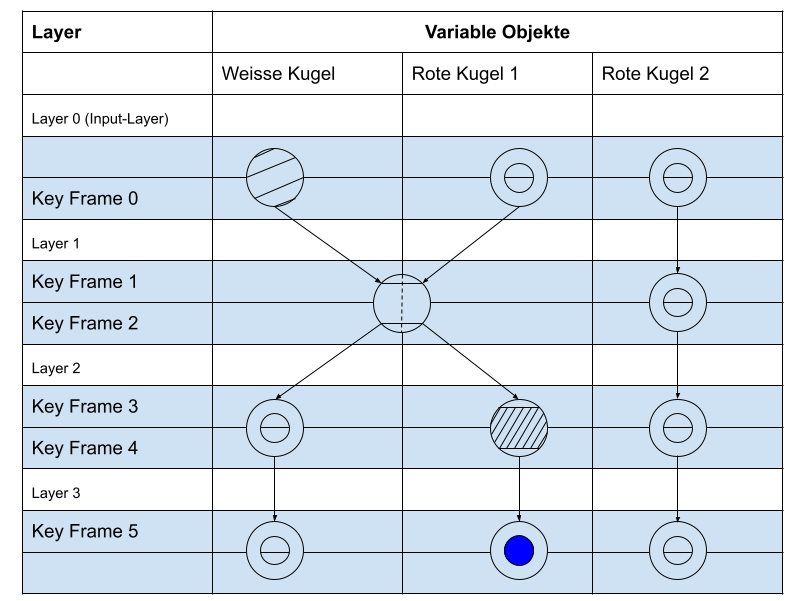
\includegraphics[width=0.6\linewidth]{../common/03_billiard_ai/resources/18_animation_keyframes.png}
    \end{center}
    \caption{Simulationsmodell mit Keyframes}
    \label{fig:simulationsmodell_keyframes}
\end{figure}

Jede Eingabe- wie auch Ausgabeschicht bildet so im Animationsmodell ein Keyframe. Die Besonderheit liegt darin, dass
nicht wie bei einer nach Lehrbuch aufgebauten Keyframe-Animation mit Fortlaufen der Zeit die Keyframes durchiteriert
\footnote{Durchiterieren bedeutet, dass wenn ein Keyframe vorher das Ende markierte, wie es das Keyframe 2 in Abbildung \ref{fig:keyframe_animation} tut, dann wird
das Keyframe 2 mit Fortlaufen der Zeit zum Startkeyframe und das nächstfolgende zum neuen Ende.} werden. Die Keyframes, welche aufgrund
des Simulationsmodells generiert werden, werden paarweise als Fenster betrachtet. Dieses Paarfenster wird bei Erreichen
des Endkeyframes auf das nächste Paar verschoben. Die Funktionsweise ist in Abbildung \ref{fig:simulationsmodell_keyframe_paare}
beschrieben. Dort werden die verschiedenen Keyframefensterpaare unterschiedlich rot markiert. Die Zeit schreitet wiederum in
vertikaler Richtung nach unten voran, der rote Pfeil auf der linken Seite zeigt eine mögliche aktuelle Position innerhalb
einer Animation. Demnach wäre das zweite Keyframefenster mit den Keyframes 2 und 3 aktiv.

\begin{figure}[h!]
    \begin{center}
        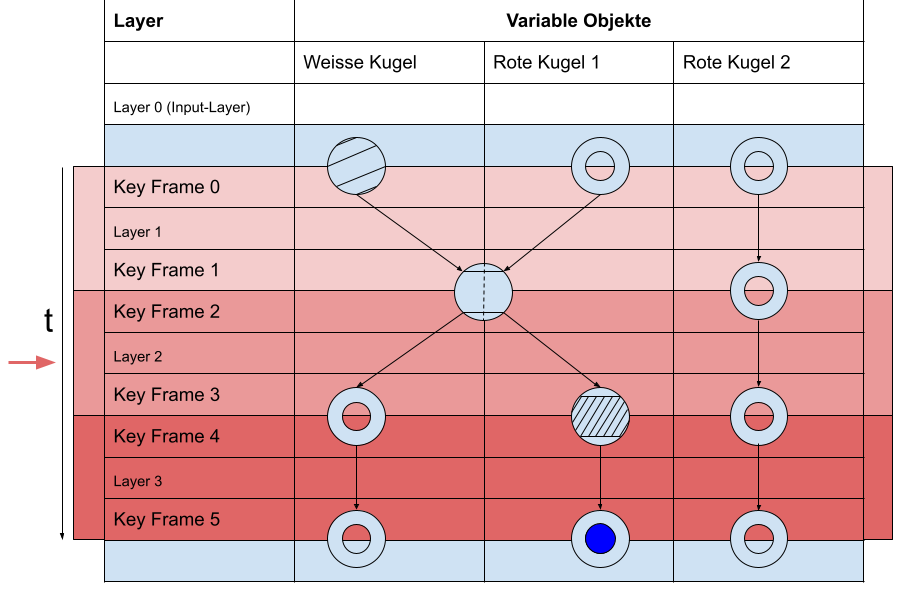
\includegraphics[width=0.6\linewidth]{../common/03_billiard_ai/resources/32_simulation_animationfenster.png}
    \end{center}
    \caption{Simulationsmodell mit paarweisen Keyframefenstern}
    \label{fig:simulationsmodell_keyframe_paare}
\end{figure}

Die Begründung der etwas spezielleren Handhabung liegt an der Tatsache, dass bei einem physikalischen Ereignis wie
einer Kugelkollision eine Veränderung des Status geschieht. So werden im Wesentlichen die Magnituden wie auch die
Richtungen der Geschwindigkeitsvektoren verändert. Würde nur ein Keyframe bei einem solchen Ereignis generiert werden,
dann könnte nicht mehr zwischen den Geschwindigkeitsvektoren aufgrund der geänderten Richtung interpoliert werden.

Die so generierte Animation kann als Gruppierung von einzelnen Keyframeanimationen, wie in Abbildung \ref{fig:keyframe_animation}
angegeben, mit jeweils nur zwei Keyframes angesehen werden.